% http://127.0.0.1:5500/openup/practice.mgmt.project_process_tailoring.base/guidances/templates/development_case_8814F1C0.html
% http://127.0.0.1:5500/openup/practice.mgmt.project_process_tailoring.base/guidances/examples/development_case_project_BA55BE59.html
\section*{Introduction}

% [The introduction of the Development Case provides an overview of the entire document. It includes the purpose, scope, definitions, acronyms, abbreviations, references, and overview of this Development Case.]
% [A introdução do Caso de Desenvolvimento fornece uma visão geral de todo o documento. Inclui o propósito, escopo, definições, acrônimos, abreviações, referências e visão geral deste Caso de Desenvolvimento.]

% Este é um projeto de um sistema de aluguel de imóveis, tendo por objetivo desenvolver uma web aplicação para gerenciamento de imóveis a serem alugados, 
% tais como os respectivos contratos de aluguel, possibilitando aos usuários rápido acesso a todoas as informações referentes aos seus imóveis e contratos em uma única plataforma. 

% A aplicaÇão consistirá de uma página web (SPA) com acesso a um servidor de dados (Backend) que deverá gerir e controlar o banco de dados de cadastro da aplicação, tal como o acesso aos usuários e os dados pessoais de usuários.

% A arquitetura básica da aplicação será feita em sistema de micro serviços, onde os micro serviços serãos separados por Domain.

% A arquitetura interna de cada micro serviço será feita em DDD seguindo os princípios do S.O.L.I.D.

% Cada Micro Serviço será uma RESTFull web api. 

\subsection*{Purpose}
% [Specify the purpose of this Development Case.]

% Reunir a informações básicas do Desenvolvimento do projeto do OpenRent e facilitar a busca por informações específicas.

Este documento descreve o processo seguido pelo projeto do OpenRent.

% \subsection*{Scope}
% [A brief description of the scope of this Development Case; what Project(s) it is associated with and anything else that is affected or influenced by this document.]

\subsubsection*{Definitions, Acronyms, and Abbreviations}
% [This subsection provides the definitions of all terms, acronyms, and abbreviations required to properly interpret the Development Case. This information may be provided by reference to the project's Glossary.]

Veja o Glossario para uma lista completa dos termos  usados nesse projeto. 

% \subsubsection*{References}
% [This section is optional. Alternatively to having an explicit references section using the table below, write down the full name of the document you are referring to in-line with the text where if first appears, then add a hyperlink to the location where the referenced element is stored, and add a acronym (between parenthesis) right after the first appearance of that reference. On subsequent appearances of that reference, use the acronym only.

% If you use this section, provide a complete list of all documents referenced elsewhere in the Development Case. Identify each document by title, report number (if applicable), date, and publishing organization. Specify the sources from which the references can be obtained. This information may be provided by reference to an appendix or to another document.

% NOTE: Be sure to include a reference to the version of the organizational process this development case is based on.]

% \begin{tabular}{|c|c|c|}
%     \hline
%     Reference Name & Owner/Author & Where Stored\\ \hline
%     && \\ \hline
%     && \\ \hline
%     && \\ \hline
%     && \\ \hline
% \end{tabular}


% [Source Process: Identify the process you are using as the base for this development case.]

% [Identify the Work Products Addendum to this development case - if addendum is used.]
 	
\subsubsection*{Overview}
% [This subsection describes what the rest of the Development Case contains and explains how the document is organized.]

O projeto do OpenRent será disciplinado mediante organização de metodologia ágil Scrum.

A equipe de Desenvolvimento está dividida em desenvolvedores, arquitetos, testers e analistas de requisitos.

% \section*{Overview of the Development Case}

\subsubsection*{Lifecycle Model}
% [Briefly describe the lifecycle model employed by the project including descriptions of the milestones and their purpose. The purpose is to serve as an introduction to the rest of the development case, not to be a project plan.]

O Desenvolvimento será feito mediante modelo iterativo, que pode ser visto na imagem \ref{fig:life_cycle}.

\begin{figure}
    \centerline{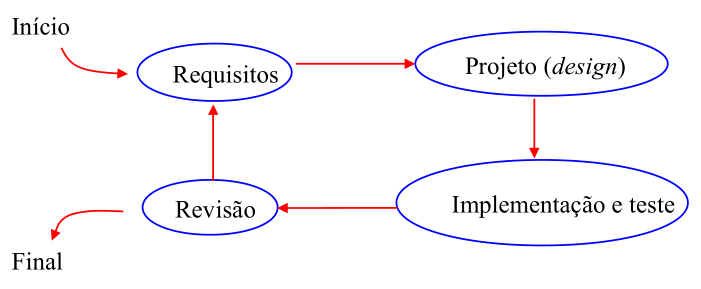
\includegraphics[width=.5\linewidth]{images/life_cicle.png}}
    \caption[Life cycle]{Modelo do ciclo de vida iterativo}
    \label{fig:life_cycle}
\end{figure}

Onde início marca o início de uma nova Sprint, prazo médio de 15 dias, sendo a sprint desenvolvida em 4 fases:
\begin{itemize}
    \item Requisitos
    \item Design e arquitetura
    \item Implementação
    \item Revisão e teste
\end{itemize}
onde essas 4 fases ocorrem de modo paralelo com cada equipe específica desenvolvendo a sua tarefa, de modo que um ciclo de Desenvolvimento completo e composto de 4 sprint sucessivas, sendo que ao final do ciclo completo se espera que seja colocado em produção a parte desenvolvida durante a sprint.

% \subsubsection*{Sample Iteration Plans}
% [This section is optional. Include sample iteration plans if they will be helpful for your project.

% Your organizational process captured in Method Composer may provide capability patterns that can serve as templates for phase iteration plans. Your organization may have included a delivery process in your published version of the organizational process that can serve as a basis for your iteration plans.

% If you are using a separate project management tool to create project plans, this section is not needed.]

% \subsubsection*{Inception Phase}
% [List the sample iteration plans used during Inception.]

% \subsubsection*{Elaboration Phase}
% [List the sample iteration plans used during Elaboration.]

% \subsubsection*{Construction Phase}
% [List the sample iteration plans used during Construction.]

% \subsubsection*{Transition Phase}
% [List the sample iteration plans used during Transition.]

\section*{Workflow}
% [This section describes the workflow of each of the development phases in your project lifecycle. 
% For each phase, identify or describe the standard workflow that is used on this project. 
% Following are some suggested ways to identify or describe the standard workflow:
%     The delivery process in your published organizational process includes activity diagrams for each development phase. 
%     You can copy and paste those diagrams here or describe how to locate them. 
%     Use the 'Notes on Workflow' section to document differences for your project.
% More difficult: 
%     rework the activity diagrams to accurately reflect the workflow that your project follows. 
%     In this case, there is no need for the 'Notes on Workflow' section, so it can be removed.]

\subsection*{Fase de Requisito}

Desenvolvido pela equipe de analistas de requisitos em conjunto com o cliente, verificando-se todos os requisitos e problemas a serem resolvidos durante a sprint. 

Nesta fase é desenvolvida protótipos de telas, verificado a interaçao do usuário. 

Também é descrito com cuidado todos os casos de uso e histórias de usuário. 
% \subsubsection*{Notes on Inception Phase Workflow}
% [Describe any changes made to the standard workflow for this phase. Typical changes include adding or removing activities or tasks to describe project-specific ways of working.]

\subsection*{Fase de Design e arquitetura}

Desenvolvido pela equipe de arquitetura, a partir das especificações da equipe de requisitos. 

Nesta fase é desenvolvida os diagramas de classe, diagramas de fluxo e pseudo código de regras de negócios específicas a serem desenvolvidas, preferêncialmente demonstando a completude e corretude do código quando possível e necessário. 

% \subsubsection*{Notes on Elaboration Phase Workflow}
% [Describe any changes made to the standard workflow for this phase. Typical changes include adding or removing activities or tasks to describe project-specific ways of working.]

\subsection*{Fase de Implementação}

Fase realizada pela equipe de Desenvolvimento frontend e backend em conjunto.

Nesta fase é implementado os diagramas de classe e de fluxo Desenvolvido pela equipe de arquitetura e também é implementado em código os pseudo código de negócios.


% \subsubsection*{Notes on Construction Phase Workflow} 
% [Describe any changes made to the standard workflow for this phase. Typical changes include adding or removing activities or tasks to describe project-specific ways of working.]

\subsection*{Fase de Revisão e teste}

Fase realizada pela equipe de teste, documentação e revisão.

Nesta fase e realizado teste intensos de cada aspecto do código desenvolvido pela equipe de desenvolvimento. 

É implementado testes automatizados para serem executados durante as fases seguintes de desenvolvimento e implementação.

É realizado a documentação do sistema, tal como manual de usuário.

Por fim é realizado a revisão do sistema e caso seja aprovado deve ser colocado em produção, e o que não foi aprovado deve ser enviado reparado na proxima sprint de desenvolvimento. 

% \subsubsection*{Notes on Transition Phase Workflow}
% [Describe any changes made to the standard workflow for this phase. Typical changes include adding or removing activities or tasks to describe project-specific ways of working.]

% \section*{Work Products}
% [A work product is an artifact, outcome, or deliverable. Provide a list of work products to be produced for the project, when the work product is created and completed, along with details of how the work product is reviewed (when appropriate), who reviews and approves the work product (RACI responsibility matrix) what template is used to create the work product, where the work product is kept or what tool is used to manage it. This can be accomplished by embedding a work product addendum to the development case, such as in spreadsheet format. Alternatively, you may use another method to provide the list of work products, either in this document or as an addendum to this document.

% Note that if you keep the work products to be produced separately from this document (for example, using an addendum spreadsheet), you must be sure to maintain proper document control of the information.]

% NOTE: The work product addendum is considered to be a part of this development case. The two documents are reviewed and approved as if they were one document.


% \section*{Reports}
% [List any reports that are useful for this project. Describe who uses the report and how it can be created.]

% \begin{tabular}{|c|c|c|}
%     \hline
%     Report & Audience & How Created/ Where Stored\\ \hline
%     && \\ \hline
%     && \\ \hline
%     && \\ \hline
%     && \\ \hline
% \end{tabular}

% \section*{Roles}
% [This section is used for the following purposes:

% To describe any changes in the set of roles; for example, it is common to refine the role stakeholder into more than one role.
% To map job positions in the organization to the roles in the organizational process. The reason for this is that in some development organizations there are job positions defined. If these job positions are commonly used and have a wide acceptance within the organization, it may be worth doing a mapping between the roles in the process and the job positions in the organization. Mapping job positions to roles makes it easier for people in the organization to understand how to employ the process. The mapping can also help people understand that roles are not job positions, a common misconception.
% Explanation of columns:

% Role: Identify the roles used on your project. For example, it is common to refine the role stakeholder into more than one role. You might need to add new roles or clarify how each role is used in the organization by providing role names commonly used in your organization
% Process Role: Y if this is a role identified in the organizational process; N if it is not defined in the process.
% Applicability: Use this column to map job positions in the organization to the roles in the organizational process.
% Responsibilities: Describe any differences in responsibilities in the organization from those described in the process.]
% NOTE: The assignment of specific individuals to particular roles or job positions is documented in the Project Plan.

% \begin{adjustbox}{width=\textwidth}
% \begin{tabular}{|c|c|c|c|}
%     \hline
%     Role&  Process Role & Applicability  &Responsibilities Different from Process \\ \hline
%     &&& \\ \hline
%     &&& \\ \hline
%     &&& \\ \hline
% \end{tabular}
% \end{adjustbox}

 	 
% \section*{Project-Specific Guidelines and Procedures} 	 
% 7. 
% [Identify any guidelines and procedures used by the project that are not included in the organizational process. These should include any special review procedures, style or coding guidelines, etc. Modify the suggested table to fit your needs.]

% \begin{tabular}{|c|c|c|c|}
%     \hline
%     Guideline or Procedure& Owner  & Used by  & Where Stored\\ \hline
%     &&& \\ \hline
%     &&& \\ \hline
% \end{tabular}
